\documentclass[a4paper,12pt]{article}

\usepackage{times}
\usepackage[french]{babel}
\usepackage[utf8x]{inputenc}
\usepackage[T1]{fontenc}
\usepackage{amsmath}
\usepackage{amssymb}
\usepackage{graphicx}
\usepackage{pdfpages}
\usepackage{pdflscape}
\usepackage{listings}
\usepackage{longtable}
\setlength{\topmargin}{0cm}
\setlength{\headsep}{0.1in}
\setlength{\headheight}{10 pt}
\setlength{\evensidemargin}{0cm}
\setlength{\oddsidemargin}{-1cm}
\textwidth 18cm
\textheight 25cm


\usepackage{fancyhdr}
\pagestyle{fancy}
\fancyhf{}
\lhead{\scriptsize{\bsc{Projet Logiciel Transversal}}}
\rhead{\scriptsize{Les Dee \& Di}}
\renewcommand{\footrulewidth}{0.5pt}
\rfoot{\scriptsize{\bsc{Ayroles}, \bsc{El Bèze}, \bsc{Maerten}}}
\lfoot{\thepage}
\lstset{literate=
{é}{{\'e}}1
{è}{{\`e}}1
{ê}{{\^e}}1
{à}{{\`a}}1
{â}{{\^a}}1
}
\lstset{language=C++,
                basicstyle=\footnotesize,
                keywordstyle=\footnotesize\color{blue},
                otherkeywords={override,nullptr}
}
\definecolor{orange}{rgb}{0.8,0.4,0.0}
\definecolor{darkblue}{rgb}{0.0,0.0,0.6}
\definecolor{cyan}{rgb}{0.0,0.6,0.6}
\lstdefinelanguage{JSON}
{
  basicstyle=\normalsize,
  columns=fullflexible,
  showstringspaces=false,
  commentstyle=\color{gray}\upshape,
  morestring=[b]",
  morestring=[s]{>}{<},
  morecomment=[s]{<?}{?>},
  stringstyle=\color{orange},
  identifierstyle=\color{darkblue},
  keywordstyle=\color{blue},
  morekeywords={string,number,array,object}% list your attributes here
}


\sloppy



\begin{document}

\renewcommand{\labelitemi}{$\bullet$}

\thispagestyle{empty}

\title{\large Projet Logiciel Transversal\\[0.5cm]
        \bf\Large Les Dee \& Di}
\author{\large \bsc{Ayroles} Quentin, \bsc{El Bèze} Ilan, \bsc{Maerten} Eloïse}
\date{2021 - 2022}
\makeatletter
    \begin{titlepage}
        \begin{center}
        \vbox{}\vspace{5cm}
            {\@title }\\[3cm] 
            {\@author}\\
            %{Instructor: \bf instructor name}\\
%            \vfill \includegraphics[scale=0.3]{images/logo.png}\\[1cm]
            {\@date}
        \end{center}
    \end{titlepage}
\makeatother
%\thispagestyle{empty}


\clearpage

{\small
\tableofcontents
}



\clearpage
\section{Présentation Générale}

\subsection{Archétype}
L’objectif de ce projet est la réalisation d’un jeu de rôle (RPG) classique inspiré par Donjons \& Dragons.

\subsection{Règles du jeu}
Le but du joueur est de réaliser la quête définie en début de partie. Pour cela il dispose d'une équipe de 6 héros avec 6 rôles différents (Guerrier, Magicien, Assassin, Archer, Druide, Prêtre). Si le joueur est seul, il joue les 6 héros. En cas de multijoueur le joueur joue les classes qu'il choisit en début de partie (il y a donc au maximum 6 joueurs sur la même partie, si le nombre de joueurs est inférieur à 6, certains joueront plusieurs héros). Le multijoueur sera donc coopératif. Les joueurs évoluent sur une carte (sous forme de grille). Sur la carte, les joueurs peuvent être confrontés à des ennemis, événements et réaliser diverses actions(comme lancer des sorts). Ces actions auront une part d’aléatoire pour imiter les lancer de dés du jeu original. À terme, l’idée est d’aussi permettre au joueur de collecter des objets et d'améliorer ses personnages. 

\subsection{Ressources}

\begin{figure}[hbt!]
    \centering
    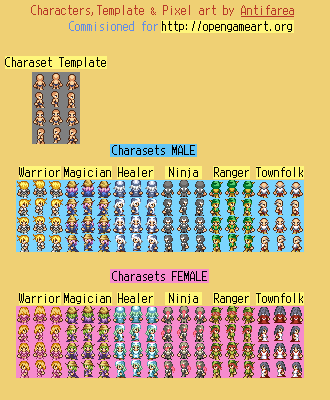
\includegraphics[scale=0.9, angle=0]{images/texture_persos1.png}
    \caption{Textures des personnages}
    \label{fig:textPerso}
\end{figure}

\begin{figure}[hbt!]
    \centering
    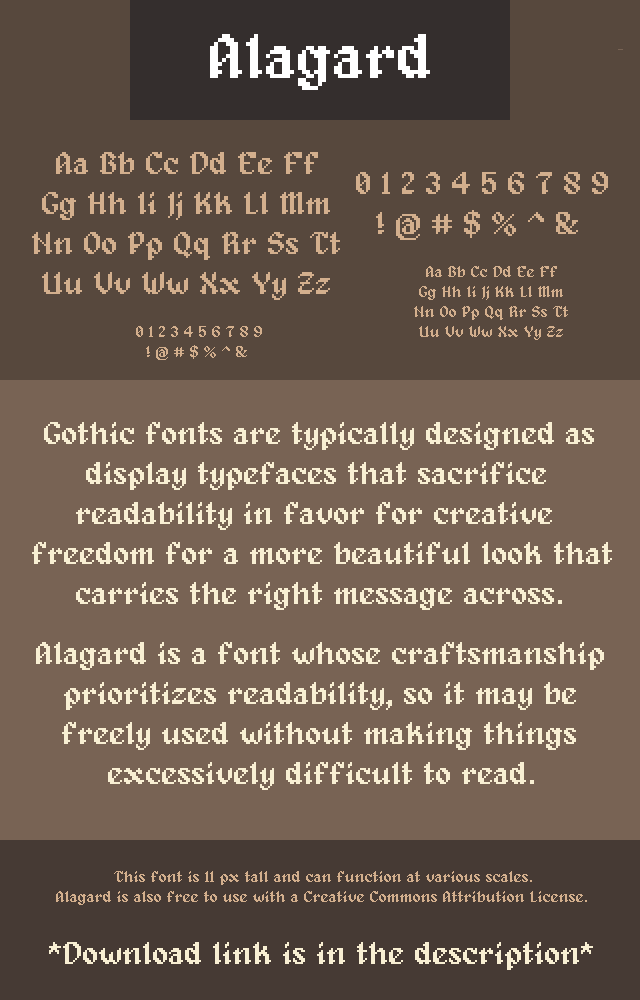
\includegraphics[scale=0.3, angle=0]{images/fonts.png}
    \caption{Police d'écriture}
    \label{fig:fonts}
\end{figure}

\begin{figure}[hbt!]
    \centering
    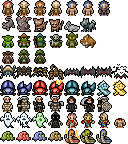
\includegraphics[scale=2, angle=0]{images/texture_monstres1.png}
    \caption{Textures des ennemies}
    \label{fig:textEnnemis}
\end{figure}

\begin{figure}[hbt!]
    \centering
    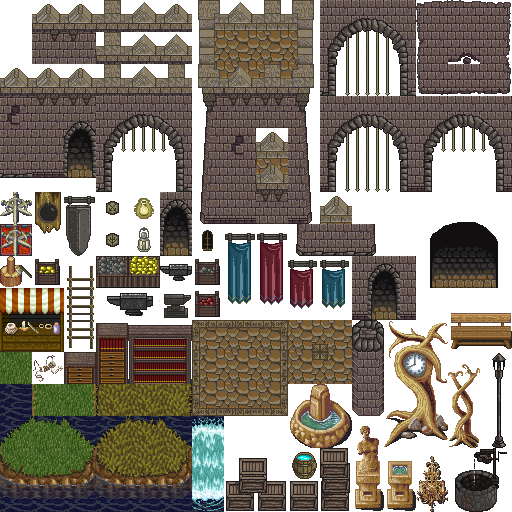
\includegraphics[scale=1.5, angle=0]{images/texture_decor1.png}
    \caption{Textures des décors}
    \label{fig:textDecor}
\end{figure}


\clearpage
\section{Description et conception des états}

\subsection{Description des états}
Un état de jeu est constitué d'un tableau d'éléments représentant la grille du jeu (donc les murs, le sol...) et un autre tableau avec les personnages (appelé entité, qui peuvent à la fois être des héros ou des ennemis). On note aussi dans l'état de jeu le nombre de tour déjà joué, ainsi que l'ordre de jeu des entités et l'entité dont c'est le tour.

\subsubsection{Éléments fixes}
La grille du plateau de jeu est constitué d'un tableau d'éléments de la classe "Décor". Un décor peut avoir un seul type parmi les suivants :

\begin{itemize}
    \item None : état passif, la case "n'existe pas" pour le joueur
    \item Mur : élément infranchissable et un obstacle visuel (on ne peut ni voir ni tirer au travers par exemple)
    \item Sol : éléments de base sur lequel le joueur peut se déplacer
    \item Porte : élément infranchissable comme le mur nécessitant une action pour s'ouvrir et se transformer en sol
    \item Secret : case porte ayant une texture de mur pouvant se révéler après une certaine action
    \item Piège : case sol infligeant des dégâts à une entité se déplaçant dessus
    \item Trésor : case sol comportant un objet (ou équipement) que le joueur peut ramasser, elle peut donc devenir une case de type sol après la récupération de l'objet
\end{itemize}

Ces éléments de décor ont donc besoin d'une méthode leur permettant de passer de leur état de "cases spéciales" (trésor, piège...) à un état de case normale tout en effectuant l'action qui leur est associé (donner un équipement pour un trésor ou infliger des dégâts pour un piège).

Chaque case est associé à un objet de la classe environnement qui définit à la fois la luminosité ambiante et la météo (neige, pluie, orage...).

Un autre argument nous permet de choisir la texture parmi une liste de textures prédéfinie nous permettant de faire varier les décors (forêt, intérieur du donjon...).


\subsubsection{Entités}
Les entités sont les personnages du jeu, qu'ils soient héros (personnages interprétés par le ou les joueurs) ou ennemis (personnages contrôlés par l'IA).Une entité possède dans sa classe toutes ses caractéristiques, comme :
\begin{itemize}
    \item niveau
    \item points de vie restants
    \item points de magie restants
    \item ses différentes statistiques comme les points d'attaque, de défense, de vitesse
    \item l'équipement qu'il possède comme des armes
    \item les statuts qu'il subit (gelé, confus...)
    \item les actions supplémentaires qu'il peut effectuer en plus de ses actions de base comme les sorts
\end{itemize}

L'ordre de jeu des entités est définie selon leur statistique d'initiative. Elle peut, durant son tour, se déplacer (selon sa statistique de déplacement) ou attaquer (selon sa statistique d'attaque). Une action supplémentaire remplace l'attaque dans son tour. Lorsque l'entité est attaqué elle se défend (selon sa statistique de défense) puis subit des dégâts et obtient possiblement un statut. Nous avons également une méthode correspondant à la mort de l'entité.

Du côté des différences entre ennemis et héros, les héros ont, en plus de ces caractéristiques, une classe (qui définit leurs statistiques de base et leur texture) et la possibilité de récupérer de l'équipement ou apprendre des actions supplémentaires comme des sorts. Les ennemis ont une race, équivalente à la classe, qui définit donc leur statistiques de base et leur textures. Pour éviter que, pendant un tour, un ennemi soit pris en compte alors qu'il n'est pas dans la même salle que les joueurs et donc pas accessible, on lui rajoute un attribut "actif" qui définit si les ennemis sont en jeu ou non. Cet attribut passe de inactif à actif lorsque le ou les joueurs sont suffisamment proche de lui.


\subsection{Conception Logiciel}

Le diagramme des classes pour les états est présenté en Figure 5, dont nous pouvons mettre en évidence les groupes de classes suivants :

Classes élément : les classes Entité, Décor, Héros, Ennemi et Équipement représentent les différentes catégories et types d'élément. Les éléments peuvent êtres séparés en trois catégories. Les éléments mobiles (Héros et Ennemi), les éléments fixes (Décor) et les éléments invisibles (équipement). Ces derniers dépendent forcément d'une Entité et ne peuvent pas exister par eux même.  

Conteneurs d’élément :  les classes State et ElementTab permettent de contenir des ensembles d’éléments. ElementTab est un tableau en deux dimension d’éléments, par exemple pour contenir la grille des éléments du niveau. Il peut également être considéré comme un tableau à une dimension dans le cas où la hauteur (height) est égale à 1 (utile pour la liste des personnages). Enfin, la classe State est le conteneur principal, à partir duquel on peut accéder à toutes les données de l’état.

\begin{figure}[hbt!]
    \centering
    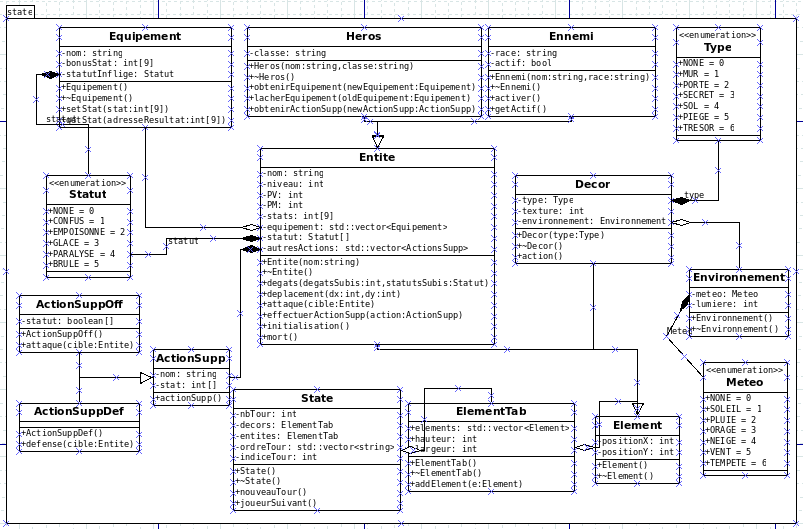
\includegraphics[scale=0.8, angle=0]{images/State_dia.png}
    \caption{Diagramme des classes d'état}
    \label{fig:diaClasseEtat}
\end{figure}


%\begin{landscape}
%\begin{figure}[p]
%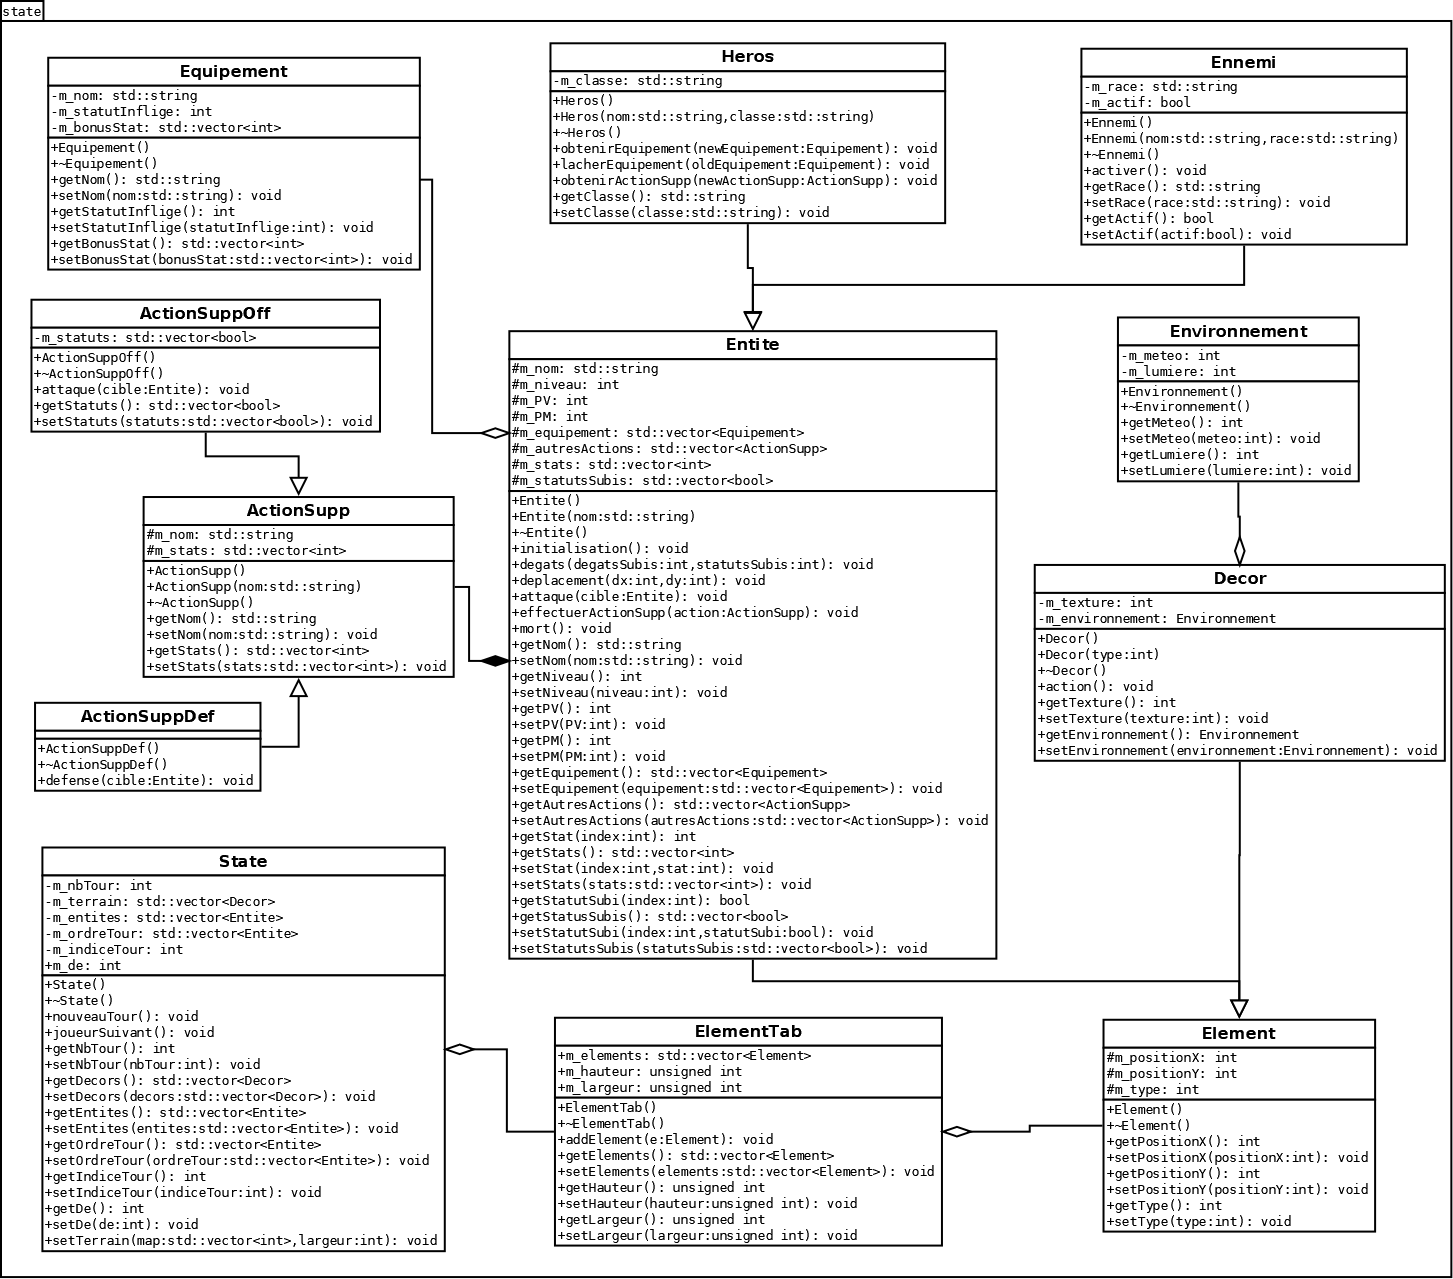
\includegraphics[width=0.9\paperheight]{state.pdf}
%\caption{\label{uml:state}Diagramme des classes d'état.} 
%\end{figure}
%\end{landscape}

\clearpage
\section{Rendu: Stratégie et Conception}

\subsection{Stratégie de rendu d'un état}


\subsection{Conception logiciel}

%\begin{landscape}
%\begin{figure}[p]
%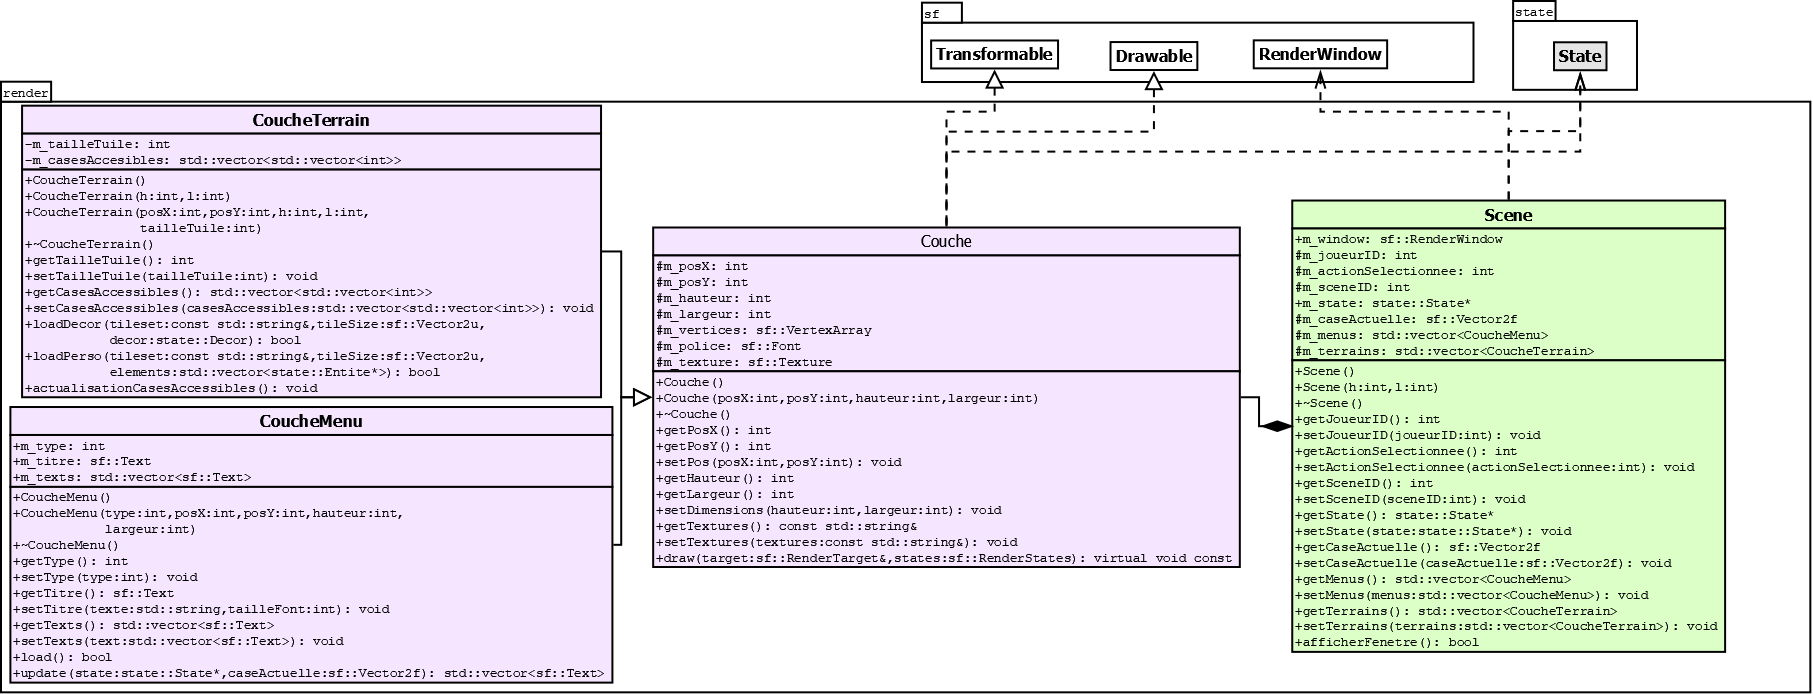
\includegraphics[width=0.9\paperheight]{render.pdf}
%\caption{\label{uml:render}Diagramme des classes de rendu.} 
%\end{figure}
%\end{landscape}

\clearpage
\section{Règles de changement d'états et moteur de jeu}

\subsection{Règles}


\subsection{Conception logiciel}


%\begin{landscape}
%\begin{figure}[p]
%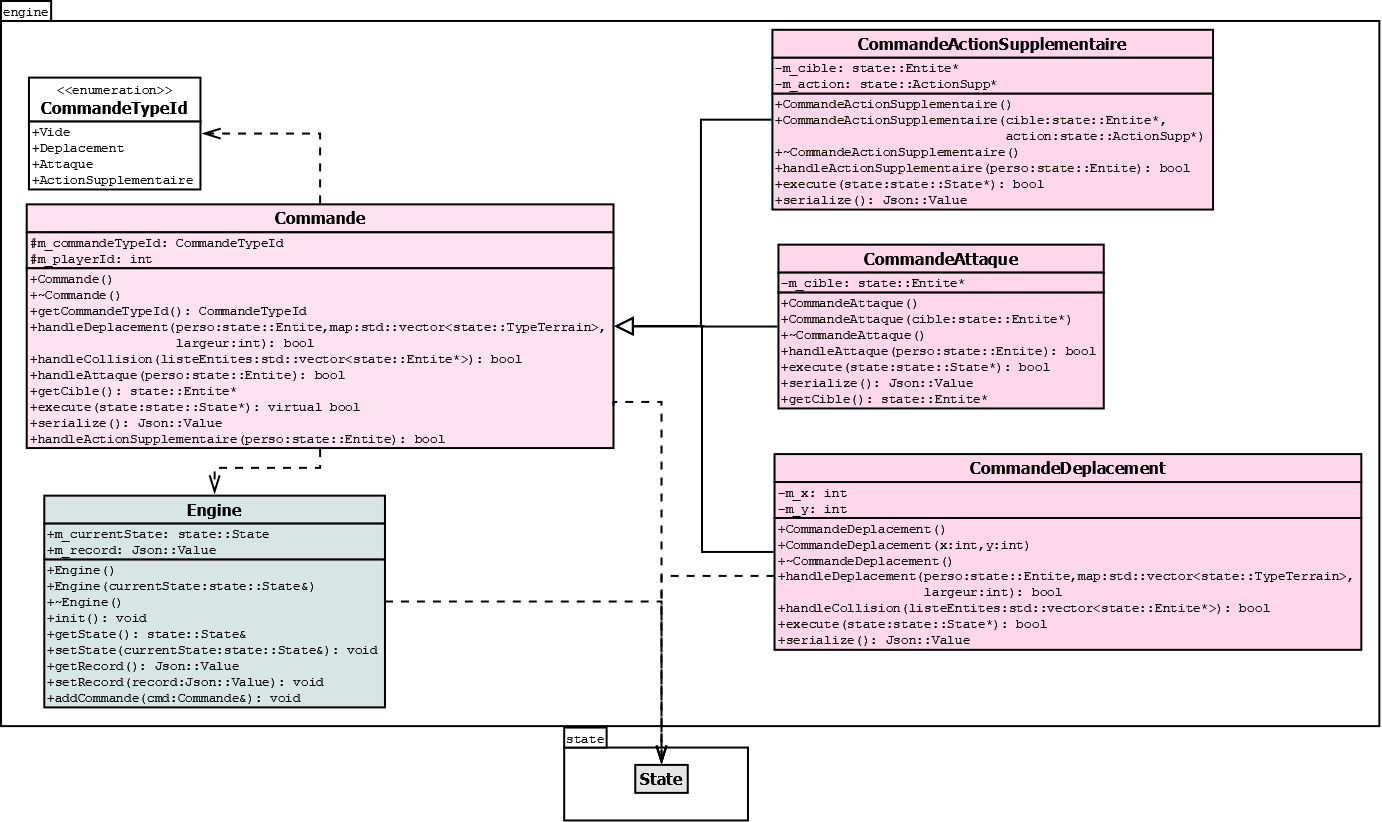
\includegraphics[width=0.9\paperheight]{engine.pdf}
%\caption{\label{uml:engine}Diagramme des classes de moteur de jeu.} 
%\end{figure}
%\end{landscape}

\clearpage
\section{Intelligence Artificielle}

\subsection{Stratégies}


\subsection{Conception logiciel}


%\begin{landscape}
%\begin{figure}[p]
%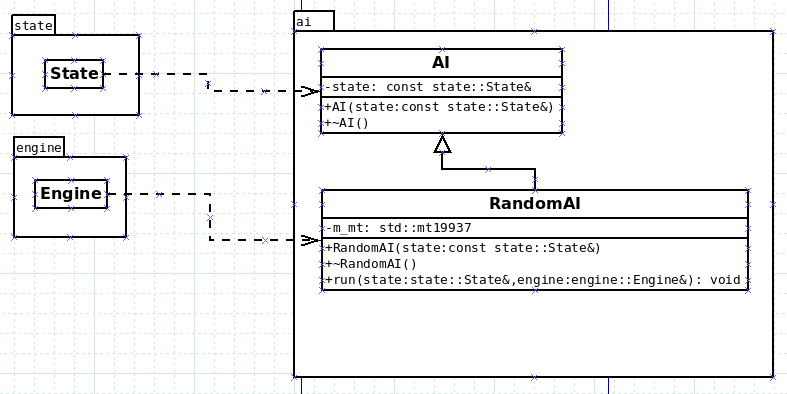
\includegraphics[width=0.9\paperheight]{ai.pdf}
%\caption{\label{uml:ai}Diagramme des classes d'intelligence artificielle.} 
%\end{figure}
%\end{landscape}

\clearpage
\section{Modularisation}
\label{sec:module}

\subsection{Organisation des modules}


\subsection{Conception logiciel}


%
%\begin{landscape}
%\begin{figure}[p]
%\includegraphics[width=0.9\paperheight]{module.pdf}
%\caption{\label{uml:module}Diagramme des classes pour la modularisation.} 
%\end{figure}
%\end{landscape}

\end{document}
